\section{Comparisons}\label{sec:comparisons}

\subsection{The published LBA97 model}
LBA97 \cite{lba97} followed the full hydrogen-burning evolution of a
$0.1\Ms$ star into white-dwarf cooling with a grey atmosphere, approximate
opacity changes as hydrogen is consumed, and the interior opacities and
reaction rates of the time. Table~\ref{tab:lba} compares their stated
values with Track P, which is the closest in physics. The starting states
are defined differently: LBA97 includes contraction and defines arrival on
the main sequence by nuclear reactions supplying the whole luminosity, after
about 2 Gyr, whereas Track P starts from a static hydrogen-burning model at
age zero. That offset is small compared with the later differences.

\begin{table}[H]\centering\small
\caption{LBA97 (literature values; curve readings marked $\simeq$) and Track P.}\label{tab:lba}
\begin{tabular}{@{}lrr@{}}\toprule
Quantity & LBA97 & Track P \\\midrule
Initial surface temperature (K) & 2228 & 2766 \\
Initial luminosity ($\Ls$) & $\simeq0.000417$ & 0.0008362 \\
Initial central density (g cm$^{-3}$) & 309 & 381.7 \\
Maximum $^3$He mass fraction & 0.0995 & 0.1003 \\
Age at maximum $^3$He (Tyr) & 1.38 & 0.7103 \\
Radiative layer first forms (Tyr; central $X$) & 5.742 ($\simeq0.16$) & 3.546 (0.1751) \\
Age at hydrogen fraction 0.2034 (Tyr) & $\simeq5.6$ & 3.40 \\
Highest surface temperature (K) & 5807 & $\geq5546$ (endpoint, still rising) \\\bottomrule
\end{tabular}
\end{table}

Ember initially radiates 2.006 times the published luminosity, and the ages
at maximum $^3$He differ by the ratio 1.943. That is what the nuclear clock
requires: with $0.07\Ms$ of hydrogen and about $6\times10^{18}$ erg g$^{-1}$
deposited, the energy supply is of order $8\times10^{50}$ erg and the
burning time is that supply divided by the mean nuclear luminosity, so a
persistently lower luminosity lengthens the clock. A homology estimate gives
the same scale. With $\rho_c\propto R^{-3}$, $T_c\propto R^{-1}$,
$\epsilon_{pp}\propto\rho T^\nu$ for $\nu\simeq4$--6, and nuclear power
equated to $4\pi R^2\sigma\Teff^4$,
\[
R\propto\Teff^{-4/(\nu+5)},\qquad
L\propto\Teff^{4(\nu+3)/(\nu+5)}\simeq\Teff^{3.1\text{--}3.3},
\]
and the temperature ratio predicts a luminosity ratio of 1.959--2.029. The
thermal times $GM^2/(RL)$ are only 3.0 and 5.5 Gyr, so a starting thermal
imbalance cannot sustain a trillion-year offset; the difference lies in the
equilibrium sequence that the physics maintains. The ratios change later in
the evolution, and no single rescaling of time aligns the two calculations.

The low LBA97 luminosity was recognized in 1997: their Section~3.1 reports a
poorer fit to the observed mass--luminosity relation than the Burrows
models. The independent solar-metallicity model of Chabrier and Baraffe
\cite{chabrier97} at $0.1\Ms$ and 1 Gyr gives 2811 K, $0.1240\Rs$ and
$0.0008511\Ls$, close to Ember; they also find that a grey Eddington
boundary generally makes low-mass models hotter, so the grey atmosphere
alone does not explain LBA97's cooler surface. Identifying the cause needs
controlled substitutions of atmosphere, opacity and equation of state, which
have not been done. A reconstruction of the original Fortran program is
available for such tests but does not reproduce LBA97: with two
low-temperature opacity choices it flags a nonconvective centre at 3.307 and
$2.946\Tyr$ (against the published 5.742), and switching only that opacity
changes its luminosity by 54.5\%. Its one close agreement, a highest surface
temperature of 5936 K against 5807 K, does not validate the rest.
Recovering Track P's photospheric density and temperature at optical depth
$2/3$ and plotting them over an opacity map, as in LBA97's Figure~6, shows
the expected drift to hotter, thinner photospheres and nothing that changes
the comparison.

The $^3$He maximum agrees to about 1\%, but Ember reaches it in half the
time and consumes hydrogen faster throughout (Figure~\ref{fig:composition}).
The HR track alone conceals this because it does not show how long the star
spends at each position. Candidate causes are the frequency-dependent
atmospheres, composition-specific opacities, the equation of state and the
updated pp rates; one-ingredient-at-a-time comparisons are needed to
separate them. Agreement with LBA97 is not a measure of accuracy.

\subsection{Independent calculations with MESA}\label{sec:mesa}
We evolved the same mass and bulk composition with the unmodified MESA
release 26.4.1 \cite{jermyn23} in two configurations. Neither shares
Ember's equation of state, opacities, network or atmosphere, so they test
whether an independent code produces the same sequence of events, not the
accuracy of any one ingredient.

\paragraph{Grey-atmosphere configuration.}
MESA starts from pre-main-sequence contraction with its supplied pp/CNO
network, OPAL and low-temperature opacities, electron conduction, an
Eddington grey atmosphere and mixing length 2. Nuclear burning reaches 99\%
of the surface luminosity at 951.3 Myr (3076 K). From that model the
evolution was continued with and without microscopic diffusion. Without
diffusion, central hydrogen crosses 0.001 at $2.372\Tyr$, the surface
reaches its maximum temperature of 6766 K at $2.406\Tyr$, and the model
cools to 595.9 K by $2.564\Tyr$, where the atmosphere requests temperatures
below the 501.2 K floor of the Ferguson opacity table. The final state has
$R=0.02572\Rs$, $L=7.516\times10^{-8}\Ls$, surface $X=0.08778$ and
$0.0009172\Ms$ of hydrogen. This is a computed cooling branch under a grey
boundary; it says nothing about that boundary's accuracy for a cold
helium-rich atmosphere. With diffusion, the same configuration reaches only
$1.225\Tyr$ (3471 K, central $X=0.4593$) in 29.91 CPU-hours: the
atmospheric equation-of-state inversion fails repeatedly on unphysical trial
pressures, a numerical fault rather than a gap along the accepted structure.

\begin{figure}[H]\centering
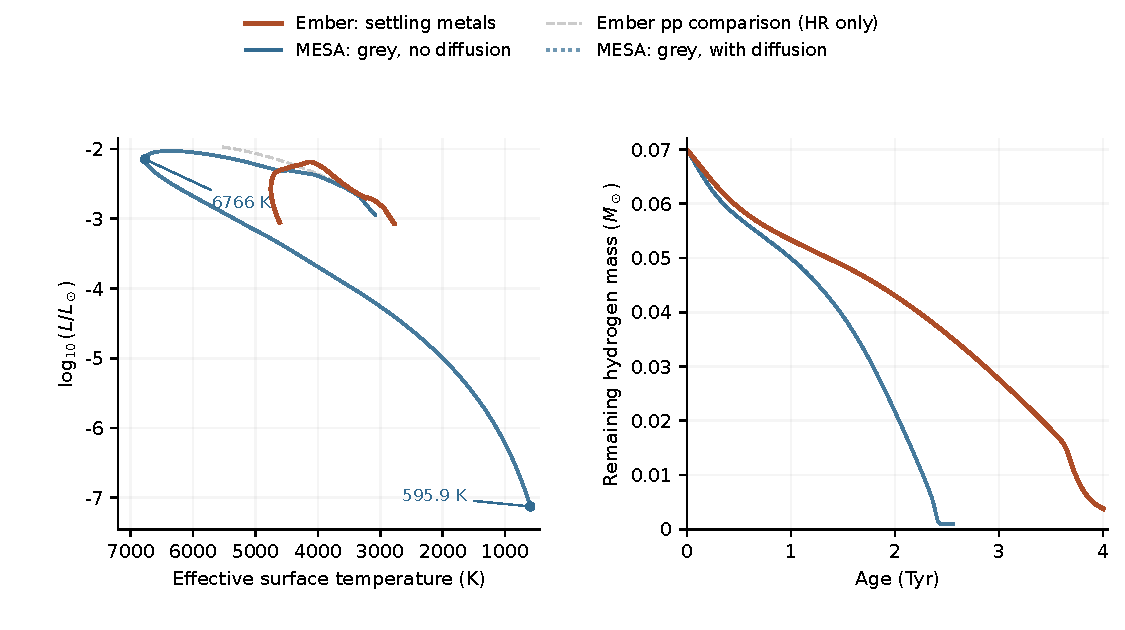
\includegraphics[width=0.85\textwidth]{mesa_comparison.pdf}\\[3pt]
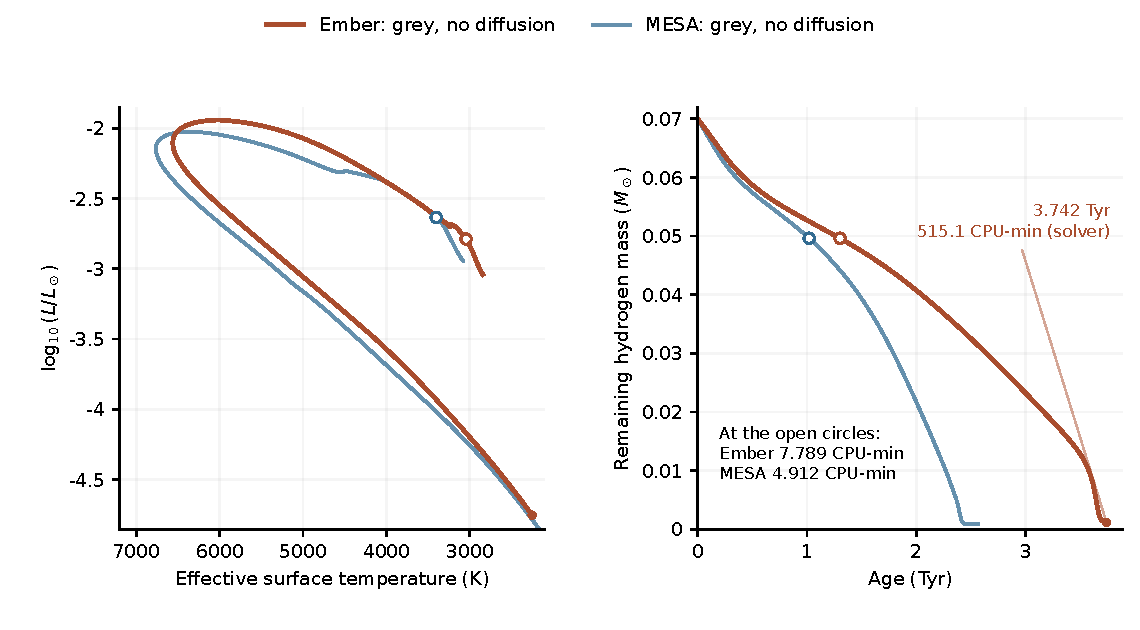
\includegraphics[width=0.85\textwidth]{grey_mesa_comparison.pdf}
\caption{Ember and MESA at $0.1\Ms$. Upper left: HR tracks, including the
computed grey MESA cooling branch; upper right: remaining hydrogen mass.
Solid blue is MESA without diffusion, dotted blue the same grey
configuration with diffusion through $1.225\Tyr$; orange is Track S and
faint dashed gray Track P. Lower: the grey-boundary comparison without
diffusion, Ember (orange, through $3.742\Tyr$) against MESA (blue); open
circles mark equal remaining hydrogen, $0.04963\Ms$, and the filled point
the last Ember model. MESA ages include contraction; Ember ages start at
the static hydrogen-burning model. Equations of state, opacities and
networks differ throughout.}
\label{fig:mesa}
\end{figure}

\paragraph{Ember with the same grey boundary.}
For a like-for-like comparison, an Ember run uses the same Eddington grey
boundary and no microscopic diffusion, with convection, pp+CN burning and
Ember's own equation of state and opacities (Figure~\ref{fig:mesa}). It
reaches $3.742\Tyr$ at 2252 K and central $X=7.991\times10^{-7}$, with a
conductive core at 1.971 MK under a convective envelope. Both codes show the
same transition when a radiative layer separates the core from the envelope:
a luminosity dip and a decline in central helium-3 once replenishment from
the envelope stops. Ember passes it at 3241 K and $3.305\Tyr$ with central
$X=0.1728$; MESA at 4498 K and $2.295\Tyr$ with $X=0.08286$. The difference
in transition temperature and composition is unexplained; the material
physics and time resolution differ, and the transients have not been
compared at matched accuracy. Below 3471 K the Ember grey run includes the
quantum correction to nuclear screening of Potekhin and Chabrier
\cite{potekhin12,chugunov09}, which changes a matched 100 Myr by 0.08920 K.
Neither this sequence nor either MESA sequence develops a helium-3 flash.

At equal remaining hydrogen ($0.04963\Ms$) Ember is at $1.302\Tyr$,
3045 K and $0.001626\Ls$, and MESA at $1.019\Tyr$, 3403 K and
$0.002316\Ls$. Their helium-3 inventories differ ($0.005740$ and
$0.003710\Ms$), so equal hydrogen does not mean equal energy released. To
that point Ember used 7.789 solver CPU-minutes and MESA 4.912 process
CPU-minutes, a ratio of 1.586; the counters have different scope, and a
fully convective phase does not measure relative cost during shell burning
or cooling. Ember's grey sequence used 515.1 solver CPU-minutes through
$3.742\Tyr$ and MESA's grey cooling sequence 1.727 CPU-hours through
750.6 K; these are different phases of different calculations and their
ratio is not a benchmark.

\paragraph{Tabulated-atmosphere configuration.}
The fuller MESA configuration uses PHOENIX and Castelli--Kurucz atmosphere
tables, OPLIB and Ferguson opacities, the blend of FreeEOS, OPAL--SCVH, HELM and Skye equations of state, conduction with the Blouin hydrogen/helium correction, 34 species with
individual diffusion, Ledoux convection with mixing length 1.9 and
Brown--Garaud--Stellmach thermohaline mixing. It has reached only 362 Myr
of contraction (2986 K). Diagnostic runs trace the slowness to diffusion
acting on the thin radiative skin above the convective envelope: when the
diffusion domain becomes active it homogenizes the skin and moves the
atmospheric boundary abruptly. Deepening the diffusion boundary to $10^5$ K
and adding a small mixing coefficient in the outer $10^{-6}$ of the mass
lets a diagnostic run continue to $2.986\Tyr$ (4694 K, central
$X=7.123\times10^{-6}$, surface $X=0.9903$) without retries. These runs
identify a numerical cause; they do not supply a physical surface-mixing
prescription and are not plotted.

A further diagnostic switched a hydrogen-rich MESA model at $3.163\Tyr$
(4737 K, $\log g=6.010$) from the grey boundary to the supplied white-dwarf
table. Within 1000 yr the photon luminosity fell by 19.96\% and the
effective temperature by 5.410\%; over the following 33.65 Myr the model
reached 4176 K with a 15.33\% larger radius. Below $\log g=6$ the MESA
wrapper blends the table with a grey boundary (22.81\% grey weight at the
endpoint), so this is not a pure table continuation. It is the same kind of
boundary change that precedes Ember's flash, and it shows that the response
is an evolving thermal adjustment rather than an equilibrium offset.

\paragraph{What the comparison establishes.}
An independent code with different physics produces the same sequence: full
convection, a radiative layer with a luminosity dip, central hydrogen
exhaustion, a temperature maximum and a turn toward cooling. The ages differ
by about a third between the codes, in the same direction as the LBA97
difference but smaller; given how strongly the nuclear clock depends on
luminosity this is expected rather than diagnostic. The 50 Gyr diffusion
comparison of Section~\ref{sec:hydrogen} shows that element redistribution,
not the omitted oxygen branches, is the stronger candidate for the late
separation between the Ember tracks, although a unique division has not been
measured. Finally, the complete pp/CNO network in MESA does not by itself
make the calculation expensive.
